\subsubsection{UC10 - Esecuzione funzione}
\begin{figure}[h]
	\centering
	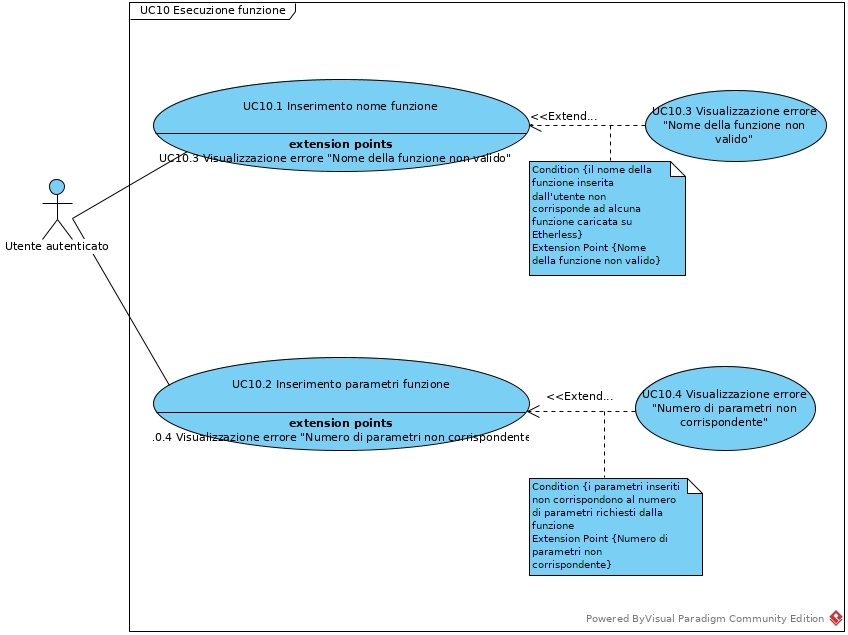
\includegraphics[width=\linewidth]{res/img/UC10.jpg}
	\caption{Diagramma UC10 - Esecuzione funzione}
\end{figure}
\begin{itemize}
	\item \textbf{Attori primari:} Utente autenticato;
	\item \textbf{Descrizione:} l'utente autenticato esegue una delle funzioni disponibili sulla piattaforma \textit{Etherless} tramite il comando "run";
	\item \textbf{Pre-condizioni:} l'utente ha effettuato l'accesso ad \textit{Etherless} e vuole eseguire una tra le funzioni messe a disposizione dagli utenti sviluppatori pagando la somma richiesta;
	\item \textbf{Post-condizioni:} il sistema visualizzerà a schermo l'output della funzione eseguita dall'utente;
	\item \textbf{Scenario principale:}
	\begin{enumerate}
		\item L'utente scriverà un comando da \textit{CLI\glo} composto nel seguente modo:
		\begin{itemize}
			\item nome del comando "run";
			\item nome della funzione;
			\item valore dei parametri.
			\item password per accedere alle credenziali salvate in locale e firmare l'avvenuta transazione.
		\end{itemize}
		\item Se il sistema non rileva errori durante dopo l'invio del comando, viene eseguito il pagamento per l'esecuzione della funzione;
		\item Il sistema, dopo aver eseguito la funzione richiesta, mostrerà sulla \textit{CLI\glo} l'output in base al valore dei parametri inseriti.
	\end{enumerate}
	\item \textbf{Inclusioni:}
	\begin{itemize}
		\item \textbf{UC11:} Ogni qualvolta l'utente esegua una funzione, deve necessariamente corrispondere il pagamento della cifra imposta dall'utente sviluppatore.
	\end{itemize}
\end{itemize}
